\chapter{Transactions}
	\section{Definition}
		\begin{itemize}
			\item Transaction resembles flow $($cash, goods, etc.$)$
			\item Transactions are the reason for business in the first place
			\item Application systems must support transaction programs!
			\item \color{red}"Transactions are the heart of economy"\color{black}
		\end{itemize}
			
	
	\section{Concept}
		\begin{itemize}
			\item A transaction is a process, that accesses and may updates data items
				\subitem databases 
				\subitem resource managers
			\item A transaction must see a consistent database at start
			\item During transaction, a database may enter a inconsistent state
			\item After the transaction is done, the Database must be consistent again
			\item There are 2 possible issues:
			\subitem Recovery $($ system crashes and similar $)$ 
			\subitem Concurrency Control $($ keeping the data consistent while multiple transactions are executed $)$
		\end{itemize}
	
	\newpage
	\section{Concurrent Executions}
		\begin{figure}[h!]
			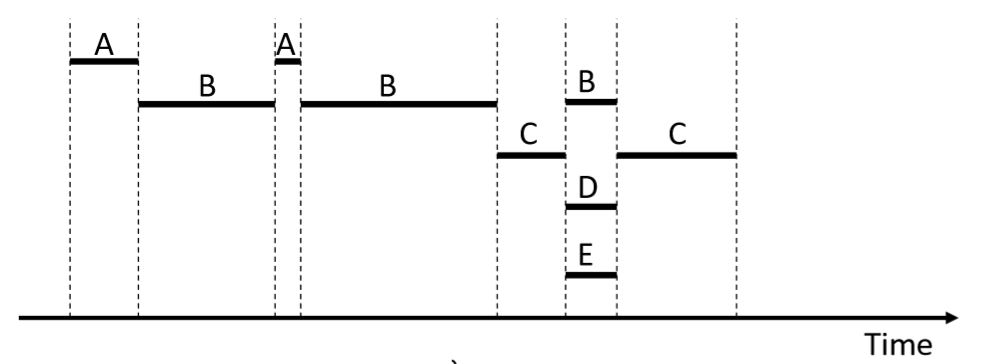
\includegraphics[scale=0.5]{res/Concurrent-Transactions.jpg}
			\caption{Types of Concurrent Transactions}
		\end{figure}
		\begin{itemize}
			\item A,B,C: Interleaved
			\item B,D,E: Simultaneous
			\item all: Parallel Transactions			
		\end{itemize}
	
	\section{Benefits of Concurrency}
		\begin{itemize}
			\item Higher Throughput
			\item More Utilization of the CPU = better value
			\item faster Response Time
		\end{itemize}
		
	\section{Possible Failures}
		
		
	\section{ACID}	
		
		
		
		
		
		
		
			
		